\section{Compilers and Interpreters}
\label{background:evaluator}

\par
Compilers and interpreters are two types of language implementation systems, and they lie at complete opposite sides of the spectrum. A third type exists, called hybrid, which merges principles of both. This chapter describes the characteristics of each. Based on this, it will argue for our choice. Finally, it will present and explain the implementation details.

The code written in our language is also called the source code. Since it is not written in machine code, the two extremes: the compiler and the interpreter, have different approaches to executing it.

\subsection{Compilers}\label{Evaluator:Compilers}
One way to execute the source code is to translate it into machine code, and this is precisely what the compiler does. Taking the source code as an input, it analyses it: first it splits it up into tokens during the lexing part, and afterwards parses the input to ensure it is properly formed as per the rules of our language. Parsing results in an abstract syntax tree, a simplified representation of the program that still contains all the important information. The semantic analyser walks the tree, verifying that the semantics are correct. Finally, machine code is generated by the code generator. During all the previous phases, the symbol table functions as a database, keeping type and attribute information for user-defined names in the program. The machine code can then be directly run by the computer, which, together with the input of the program, produces the result. The diagram at \cref{fig:compilerdiag} below illustrates this process.

\begin{figure}[!ht]
  \centering
  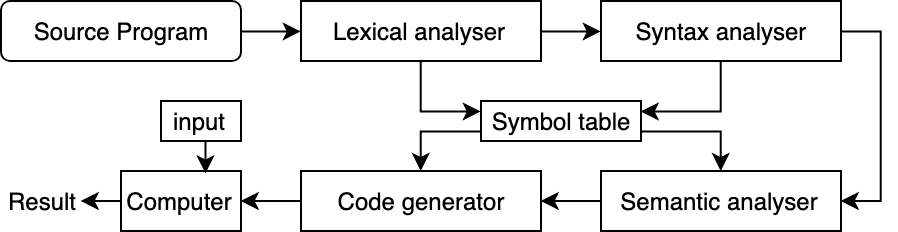
\includegraphics[scale=0.3]{Pictures/compiler-diagram.png}
  \caption{Diagram of a compiler}
  \label{fig:compilerdiag}
\end{figure}

Compiling has the great advantage of performance. After the translation process, which only needs to be performed once, execution is very fast.

\subsection{Interpreters}\label{Evaluator:Interpreters}

As mentioned before, interpreters are polar opposites of compilers as far as language implementation systems go. As opposed to compilers, which translate the source code into machine language in order for it to be executed, interpreters use the interpreter to interpret the source code directly. This can be done without having to translate the code. The interpreter can, therefore, be thought of as a virtual machine for our program.

\par
Interpreters have the advantage of an easier implementation of debugging operations since run-time is tightly knit with the source code. However, it comes at the cost of performance. Execution is 10 to 100 times slower than in compiled systems \cite[p. 50]{concepts-of-programming-languages}, which is the result of decoding the high-level statements. Space is also a disadvantage since the symbol table is needed during execution.

\begin{figure}[!ht]
  \centering
  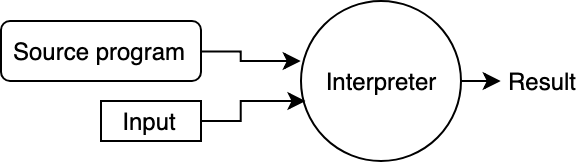
\includegraphics[scale=0.3]{Pictures/interpreter-diagram.png}
  \caption{Diagram of an interpreter}
  \label{fig:interpreterdiag}
\end{figure}

\subsection{Hybrid implementation systems}\label{Evaluator:Hybrid}
Hybrid implementation systems offer a compromise between compilers and interpreters. Hybrid implementation systems share the same front as compilers, but the intermediate code is interpreted as opposed to being translated to machine code. 

\begin{figure}[!ht]
  \centering
  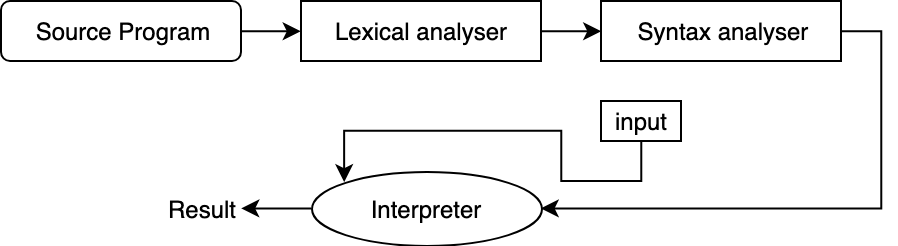
\includegraphics[scale=0.3]{Pictures/hybrid-diagram.png}
  \caption{Diagram of a hybrid implementation system}
  \label{fig:hybriddiag}
\end{figure}

